\documentclass[10pt,a4paper]{article}
\usepackage[utf8]{inputenc}
\usepackage[english]{babel}
\usepackage{amsmath}
\usepackage{amsfonts}
\usepackage{amssymb}
\usepackage{graphicx}
\usepackage[margin=0.5in]{geometry}
\usepackage{amsthm}
\usepackage{enumitem}
\usepackage{tikz}
\usetikzlibrary{calc}
\newtheorem{question}{Question}
\newtheorem*{question*}{Question}
\newtheorem{theorem}{Theorem}
\newtheorem{lemma}{Lemma}

\theoremstyle{definition}
\newtheorem{answer}{Answer}
\newtheorem*{answer*}{Answer}


\title{Complex Analysis Homework 2}
\author{Colin Williams}

\begin{document}
\maketitle
\section*{Question 2}
\begin{question*}{$ $}
\\Find all the roots in rectangular coordinates and show them on a graph. 
\begin{enumerate}[label = \alph*.)]
\item $(-1)^{1/3}$
\item $8^{1/6}$.
\end{enumerate}
\end{question*}

\begin{answer*}
Some points of note before we begin:
\begin{enumerate}[label = \roman*.)]
\item First, notice you can write any $z \in \mathbb{C}$ in rectangular coordinates as $z = x + iy$ or in polar coordinates as $z = r(cos(\theta) + i\sin(\theta))$ for $r = |z|$, $x = r\cos(\theta)$, and $y = r\sin(\theta)$. 
\item Also, note that $e^{i\theta} = \cos(\theta) + i\sin(\theta)$, so $z = re^{i\theta}$
\item Lastly, two nonzero complex numbers, $z_1 = r_1e^{i\theta_1}$ and $z_2 = r_2e^{i\theta_2}$ are equal if and only if $r_1 = r_2$ and $\theta_1 = \theta_2 + 2\pi k$ for $k \in \mathbb{Z}$.
\end{enumerate}
\end{answer*}

\begin{answer*}{\textbf{a.)}}
\\If $z_0 = -1$, then $r = |z_0| = \sqrt{(-1)^2 + 0^2} = 1$ and $\cos(\theta) = -1$ and $\sin(\theta) = 0 \implies \theta = -\pi$. Thus, $z_0 = e^{i(-\pi)}$.
\\We are looking for a $z = re^{i\theta}$ such that $z^3 = z_0$. Or,
\[r^3e^{i3\theta} = e^{i(-\pi)}\]
By $iii.)$, $r^3 = 1$ and $3\theta = -\pi + 2\pi k$.
\\$\implies r = 1$ and $\theta = -\pi/3 + (2\pi k)/3$.
\\Since $\theta$ is $2\pi$ periodic, we only have distinct values for $z$ when $k \in \{0,1,2\}$.
\\Thus, our potential values for z are:
\begin{align*}
z &\in \{e^{i(-\pi/3)}, e^{i(-\pi/3 + 2\pi/3)}, e^{i(-\pi/3 + 4\pi/3)}\}\\
&= \{e^{i(-\pi/3)}, e^{i(\pi/3)}, e^{i(\pi)}\}\\
&= \{\cos(-\pi/3) + i\sin(-\pi/3), \cos(\pi/3) + i\sin(\pi/3), \cos(\pi) + i\sin(\pi)\}\\
&= \{1/2 + i(-\sqrt{3}/2), 1/2 + i(\sqrt{3}/2), -1 + i(0)\}\\
&= \boxed{\{1/2 - i(\sqrt{3}/2), 1/2 + i(\sqrt{3}/2), -1\}}
\end{align*}

If we graph these on the complex plane, they all lie on the circle centered at $(0,0)$ with radius $1$:

\begin{tikzpicture}[scale = 2]
\draw [help lines, <->] (-2,0) -- (2,0);
\node [below right] at (2,0) {$Re(z)$};
\draw [help lines, <->] (0,-2) -- (0,2);
\node [above left] at (0,2) {$Im(z)$};
\draw [black] (0,0) circle [radius=1];
\draw[fill, red] (1/2,-{sqrt(3)/2}) circle [radius=0.05];
\node [below right, red] at (1/2,-{sqrt(3)/2}) {$1/2 - i(\sqrt{3}/2)$};
\draw[fill, blue] (1/2,{sqrt(3)/2}) circle [radius=0.05];
\node [above right, blue] at (1/2,{sqrt(3)/2}) {$1/2 + i(\sqrt{3}/2)$};
\draw[fill, violet] (-1,0) circle [radius=0.05];
\node [above left, violet] at (-1,0) {$-1$};
\end{tikzpicture}
\end{answer*}

\begin{answer*}{\textbf{b.)}}
\\If $z_0 = 8$, then $r = |z_0| = \sqrt{(8)^2 + 0^2} = 8$ and $\cos(\theta) = 1$ and $\sin(\theta) = 0 \implies \theta = 0$. Thus, $z_0 = 8e^{i0}$.
\\We are looking for a $z = re^{i\theta}$ such that $z^6 = z_0$. Or,
\[r^6e^{i6\theta} = 8e^{i0}\]
By $iii.)$, $r^6 = 8$ and $6\theta = 0 + 2\pi k$.
\\$\implies r = \sqrt{2}$ and $\theta = (2\pi k)/6$.
\\Since $\theta$ is $2\pi$ periodic, we only have distinct values for $z$ when $k \in \{0,1,2,3,4,5\}$.
\\Thus, our potential values for z are:
\begin{align*}
z &\in \{\sqrt{2}e^{i(2\pi 0)/6}, \sqrt{2}e^{i(2\pi)/6}, \sqrt{2}e^{i(4\pi)/6}, \sqrt{2}e^{i(6\pi)/6}, \sqrt{2}e^{i(8\pi)/6}, \sqrt{2}e^{i(10\pi)/6}\}\\
&= \{\sqrt{2}, \sqrt{2}e^{i(\pi/3)}, \sqrt{2}e^{i(2\pi/3)}, \sqrt{2}e^{i(\pi)}, \sqrt{2}e^{i(4\pi/3)}, \sqrt{2}e^{i(5\pi/3)}\}\\
&= \{\sqrt{2}, \sqrt{2}(\cos(\pi/3) + i\sin(\pi/3)), \sqrt{2}(\cos(2\pi/3) + i\sin(2\pi/3)), \\
&\quad \quad \sqrt{2}(\cos(\pi) + i\sin(\pi)), \sqrt{2}(\cos(4\pi/3) + i\sin(4\pi/3)), \sqrt{2}(\cos(5\pi/3) + i\sin(5\pi/3))\}\\
&= \{\sqrt{2}, \sqrt{2}(1/2 + i(\sqrt{3}/2)), \sqrt{2}(-1/2 + i(\sqrt{3}/2)), \sqrt{2}(-1 + i(0)), \sqrt{2}(-1/2 - i(\sqrt{3}/2)), \sqrt{2}(1/2 - i(\sqrt{3}/2))\}\\
&= \boxed{\{\sqrt{2}, \sqrt{2}/2 + i(\sqrt{6}/2), -\sqrt{2}/2 + i(\sqrt{6}/2), -\sqrt{2}, -\sqrt{2}/2 - i(\sqrt{6}/2), \sqrt{2}/2 - i(\sqrt{6}/2)\}}
\end{align*}

If we graph these on the complex plane, they all lie on the circle centered at $(0,0)$ with radius $\sqrt{2}$:

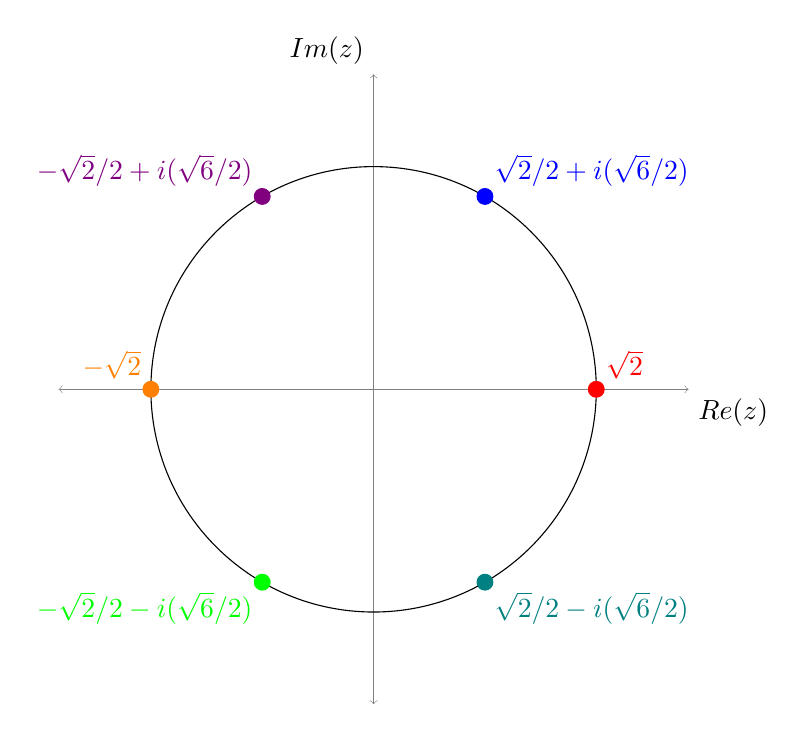
\begin{tikzpicture}[scale = 2]
\draw [help lines, <->] (-2,0) -- (2,0);
\node [below right] at (2,0) {$Re(z)$};
\draw [help lines, <->] (0,-2) -- (0,2);
\node [above left] at (0,2) {$Im(z)$};
\draw [black] (0,0) circle [radius=sqrt(2)];
\draw[fill, red] ({sqrt(2)},0) circle [radius=0.05];
\node [above right, red] at ({sqrt(2)},0) {$\sqrt{2}$};
\draw[fill, blue] ({sqrt(2)/2},{sqrt(6)/2}) circle [radius=0.05];
\node [above right, blue] at ({sqrt(2)/2},{sqrt(6)/2}) {$\sqrt{2}/2 + i(\sqrt{6}/2)$};
\draw[fill, violet] ({-sqrt(2)/2},{sqrt(6)/2}) circle [radius=0.05];
\node [above left, violet] at ({-sqrt(2)/2},{sqrt(6)/2}) {$-\sqrt{2}/2 + i(\sqrt{6}/2)$};
\draw[fill, orange] ({-sqrt(2)},0) circle [radius=0.05];
\node [above left, orange] at ({-sqrt(2)},0) {$-\sqrt{2}$};
\draw[fill, green] ({-sqrt(2)/2},{-sqrt(6)/2}) circle [radius=0.05];
\node [below left, green] at ({-sqrt(2)/2},{-sqrt(6)/2}) {$-\sqrt{2}/2 - i(\sqrt{6}/2)$};
\draw[fill, teal] ({sqrt(2)/2},{-sqrt(6)/2}) circle [radius=0.05];
\node [below right, teal] at ({sqrt(2)/2},{-sqrt(6)/2}) {$\sqrt{2}/2 - i(\sqrt{6}/2)$};
\end{tikzpicture}
\end{answer*}


\end{document}